\newsection
\subsection{Security and privacy}
\label{sec:security}
\sectionauthors{Florian Tramèr*, Rohith Kuditipudi*, Xuechen Li*}

\begin{figure}[!ht]
\centering
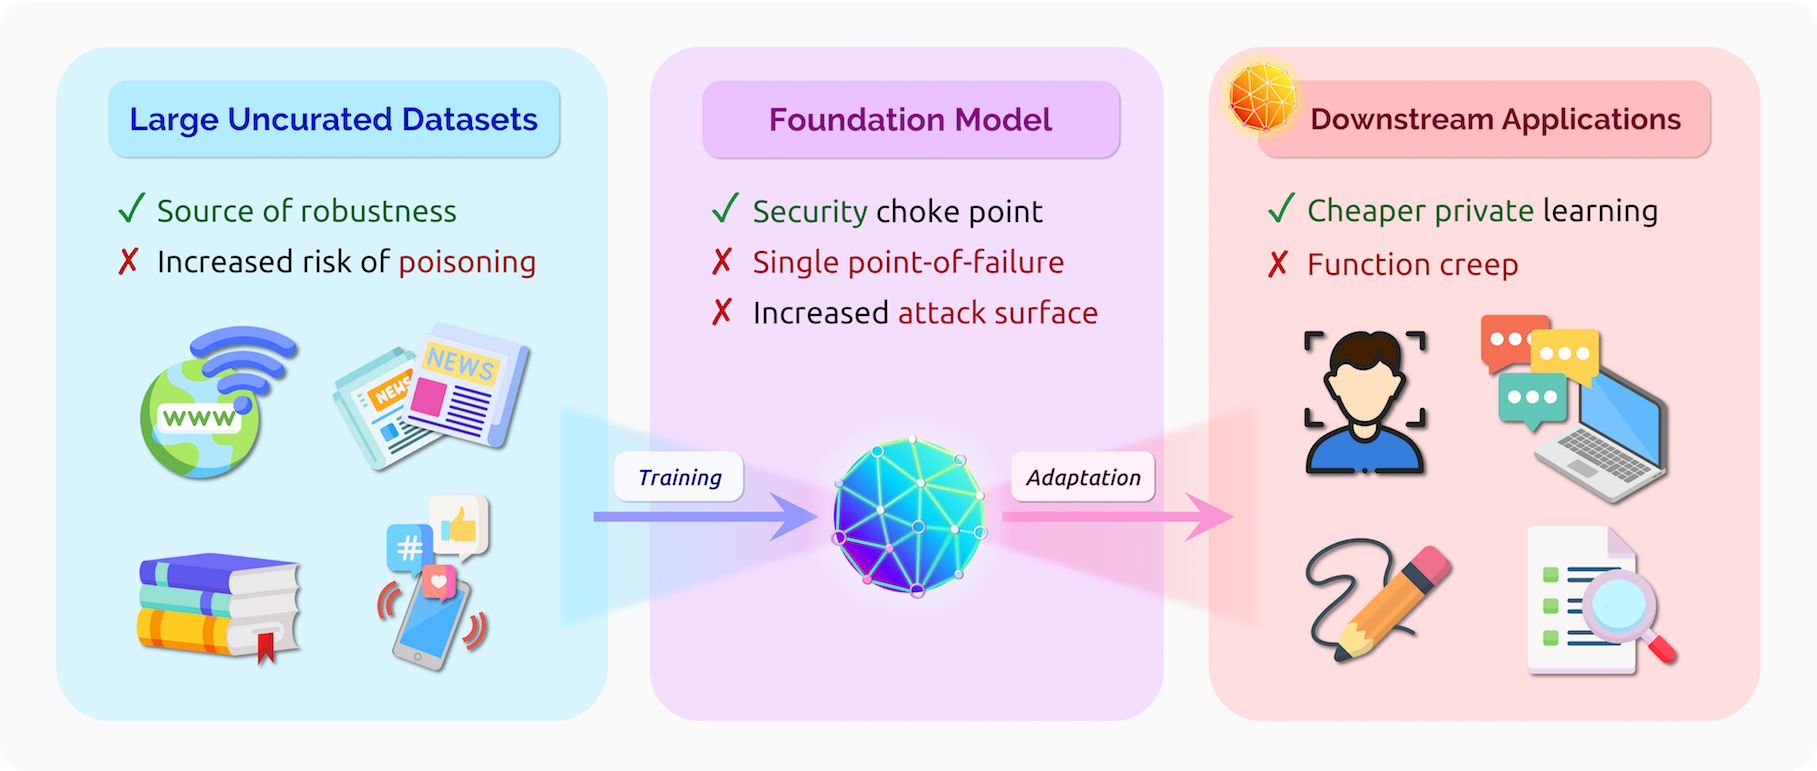
\includegraphics[width=\linewidth]{technology/figures/Security.png}
\caption{\label{fig:security} Risks and opportunities raised by foundation models for security and privacy of ML systems. 
}
\end{figure}

As central components in critical data-driven decision-making systems, machine learning models must address a variety of security and privacy threats.\footnote{In this section, we focus on \emph{security for foundation models}. Some applications of \emph{foundation models for security} (\eg detection of toxic content) are discussed in \refsec{misuse}.} These threats can be characterized using the traditional ``CIA triad'' of computer security. ML systems should protect the \textbf{Confidentiality} of user data against \emph{inference and reconstruction attacks}~\citep{fredrikson2015model,shokri2017membership, carlini2019secret, carlini2020extracting}. Moreover, the secrecy of trained models themselves can be at risk of \emph{model stealing attacks}~\citep{tramer2016stealing, papernot2017blackbox}. The \textbf{Integrity} of ML systems can be compromised by \emph{adversarial examples}~\citep{biggio2013evasion, szegedy2014intriguing} and \emph{data poisoning attacks}~\citep{biggio2012poisoning, chen2017targeted}. Finally, \emph{resource-depletion attacks}~\citep{shumailov2020sponge,hong2020panda} can threaten the \textbf{Availability} of ML systems.

In regard to these threats, we posit that the security role of foundation models in future machine learning systems will be akin to the role played by the \emph{operating system} in traditional software systems. Due to its generality and ubiquity, a foundation model may become a \emph{single point of failure} and thus a prime target for attacks against applications derived from this model.
In turn however, a foundation model imbued with strong security and privacy properties could form the backbone for the design of a variety of secure and reliable ML applications. Of course, these applications may still have to be designed to enforce specific security and privacy guarantees (in the same way that software designers cannot rely on a secure operating system to protect against all security risks).

\subsubsection{Risks}
\paragraph{Single points of failure.}
A foundation model that is adapted to a variety of applications represents a single point of failure for these applications. 
For example, data poisoning attacks on a foundation model, where an adversary inserts malicious examples into the training data, might impact all adapted applications as well. 
Similarly, adversarial examples against a foundation model (\ie small input perturbations that cause the model to output very different features) could more easily transfer to adapted applications. \citet{wallace2019universal} even find that a \emph{single} adversarial trigger added to any input can cause language models such as GPT-2 to output a predefined piece of text.
A foundation model can also become a single point of failure for data privacy.
If a foundation model is pretrained on a company's private data and the model memorizes part of this data, all downstream applications could run the risk of exposing this data \citep{carlini2020extracting}.
The provider of a foundation model may also be a single point of trust for the privacy of application data. For example, the current API for GPT-3 requires that all (potentially sensitive) data used for fine-tuning or inference be uploaded to OpenAI's servers. Designing a foundation model service that avoids this centralization of trust is an interesting problem.

If the parameters of a foundation model are public, model stealing attacks on adapted applications could be facilitated, as the attacker only needs to reverse-engineer the ``delta'' with respect to the public foundation model \citep{krishna2019thieves} (\eg a linear model trained on features extracted from a public frozen model).

Finally, denial-of-service attacks on the foundation model provider could also be a concern and might be exacerbated by querying the model with special high-cost inputs~\citep{shumailov2020sponge}.

\paragraph{Data poisoning.}
Successful foundation models have so far been trained on large and often uncurated datasets scraped from the 
Web~\citep{radford2021learning,radford2019language}. 
This permissive data collection\dash{}coupled with a lack of direct training supervision\dash{}facilitates poisoning attacks on a foundation model's training data (\eg injecting hateful speech targeted at a specific individual or company into a few outbound pages from Reddit).
Worse, the power of poisoning attacks may be exacerbated by the  growing size and accuracy of today's models~\citep{carlini2021poisoningssl}.

To illustrate, \citet{schuster2021you} show that a code auto-completion system trained with GPT-2 on Github data can be poisoned into suggesting insecure code snippets with the injection of only a few malicious files.
\citet{carlini2021poisoning} further show that targeted attacks against CLIP-style~\citep{radford2021learning} models require modifying as little as two out of 3 million training examples.


\paragraph{Function creep \& dual use.}
Foundation models learn general features that enable them to be easily adapted to a variety of tasks. 
This flexibility, however, raises  concerns that foundation models could be used beyond their originally foreseen purposes%
\dash{}a risk commonly referred to as \emph{function creep} or \emph{dual use}.
Examples of function creep in machine learning include \emph{overlearning}~\citep{song2019overlearning} and \emph{adversarial reprogramming}~\citep{elsayed2018adversarial}.

To illustrate, CLIP was originally trained to solve the generic task of predicting image-text pairs, but in doing so also learned to capture rich facial features~\citep{goh2021multimodal}. 
While CLIP's ``model card''\footnote{\url{https://github.com/openai/CLIP/blob/main/model-card.md}. Accessed 06.30.2021} explicitly places facial recognition and other surveillance technologies as out-of-scope, CLIP can certainly be re-purposed for such tasks \citep{radiya2021data}.
This example illustrates that it may be challenging to constrain (or even foresee) the possible nefarious uses of a foundation model when it is designed. \refsec{misuse} provides further discussions on dual (mis)use of foundation models.

\paragraph{Multimodal inconsistencies.}
Multimodality may increase the attack surface of foundation models, by enabling adversaries to exploit inconsistencies across modalities.
The possibility of such attacks was demonstrated in an (in)famous example of CLIP classifying an apple with the word ``iPod'' stuck to it as an iPod~\citep{goh2021multimodal}. 
More generally, whenever a concept can be expressed using different modalities, inconsistencies across these modalities may be exploitable.

Such inconsistencies are particularly concerning when a foundation model is adapted to a task that primarily relies on only one of the learned modalities. For example, consider using features extracted from CLIP for facial recognition. This is a purely visual task, yet the adapted model's features will still be sensitive to textual signals (thus, an attacker might be able to evade facial recognition by wearing clothes with imprinted text). 
Alternatively, consider an autonomous driving system (an application that also relies primarily on vision) that sees a billboard with the word ``green'' on it, and mistakenly interprets this as a green light.

\subsubsection{Opportunities}
\paragraph{Security choke points.}
If adapted applications can inherit vulnerabilities from a foundation model, they can also inherit desirable security characteristics\dash{}such as robustness to adversarial examples or poisoning attacks. Foundation models could thus serve as security \textit{choke points}.
For example, a model robust to adversarial examples can retain its robustness when it is adapted to other tasks~\citep{shafahi2019adversarially}. 
Similarly, a foundation model provider that can (somehow) defend against poisoning, model-stealing or resource-depletion attacks could then provide such security guarantees for its customers' applications.

The tradeoff between a foundation model's role as a single point of failure or as a security choke point is reminiscent of similar security tradeoffs in other \emph{abstraction layers} in the software stack (\eg an operating system, database system, or a Web browser). By virtue of serving many different applications, an abstraction layer is a prime target for attack, but can typically also leverage far greater resources to enhance its security compared to any single application.

\paragraph{Cheaper private learning.}
Current foundation models are often trained by amassing vast amounts of data from publicly available sources (\eg from the open Web). 
This practice may raise concerns about privacy\dash{}in the broad sense of taking user data out of its intended context~\citep{nissenbaum2004privacy, carlini2020extracting}. Yet, it could also end up being a \emph{win} for user privacy in applications that handle scarce and sensitive data (\eg in healthcare). 

As an example, consider the problem of training a \emph{differentially private} model~\citep{dwork2006calibrating} for a healthcare task. Training such a model ``end-to-end'' (\ie without leveraging any pretraining) to a decent privacy-utility tradeoff currently requires vast amounts of privacy-sensitive data~\citep{mcmahan2017learning, basu2021benchmarking}. In contrast, a foundation model pretrained on public data could potentially be adapted to the specific healthcare task 
with significantly less confidential data~\citep{bommasani19towards, tramer2021dp}.

\paragraph{Robustness to adversarial examples at scale.}
There is evidence suggesting that training a model that is robust to adversarial examples requires vastly more data compared to standard training \citep{schmidt2018adversarially}, but that unlabeled data may suffice to bridge this gap \citep{carmon2019unlabeled,uesato2019are}.
Moreover, increasing model size and capacity (\ie over-parameterization) has also been shown to be necessary for achieving adversarial robustness in some settings \citep{madry2018towards,bubeck2021universal}.
Understanding how best to leverage over-parameterization and unlabeled data to achieve adversarial robustness is an important direction for future research. Given their unprecedented scale (both in terms of model size and training set size),
foundation models are uniquely positioned to benefit from this line of inquiry.

Despite their unprecedented scale, current foundation models unfortunately see little gains in robustness to worst-case adversarial perturbations~\citep{Fort2021CLIPadversarial, wallace2019universal}. However, multimodal models such as CLIP are surprisingly robust to (non-adversarial) distributional shifts (see \refsec{robustness}).
Whether these gains in distributional robustness can translate to increased resilience 
against real-world attacks is another exciting open question.
Particularly in settings where adversaries are subject to various constraints (\eg limited query access or computational budget), there is reason to be optimistic that enhanced distributional robustness could lead to concomitant gains in overall security\dash{}even if the foundation model remains vulnerable to worst-case ``white-box'' attacks. 